\documentclass{article}
\usepackage{graphicx}
\usepackage{threeparttable}
\usepackage{amssymb}
\usepackage{hyperref}

\usepackage{pdflscape}

\title{Concepts of function in biology and biomedicine}

\begin{document}
\maketitle

\section{Abstract}
\label{sec:abstract}

Several philosophical accounts of disease are constructed at least partly around an objective biological criterion. Under these accounts, we can define disease as the failure of physiological parts or processes to perform their proper function or an ``impairment of normal functioning''. Determining whether a phenotype—such as obesity—is a disease or determining the level of functioning at which some aspect of physiology—such as response to insulin—becomes pathological throws considerable weight on the concept of biological function. However, there are a number of philosophical theories of function, each of which defines function differently. It is not clear which theory—or combination of theories—we should use to explicate the medical conception of function. One reason for this is that we have no systematic way to determine how biologists and medical practitioners conceive of, or write about, function in their respective disciplines. To further complicate matters, natural language is replete with ambiguities, and scientific manuscripts often use technical terms imprecisely. Without a descriptive understanding of how different conceptions of function are used in biology and medicine, we have little hope of bringing insights on biological function to bear on disputes about function and malfunction in medicine. Here we develop a systematic method for analysing biological function by outlining a classification scheme that combines syntactic and semantic analysis in a dependency-grammar framework.

\section{Introduction}
\label{sec:introduction}

Much of philosophy of medicine is concerned with defining issues surrounding the concept of disease.
Philosophical approaches to categorising disease can be broadly divided into two camps: a constructivist view that prioritises social value judgements and a naturalist view that prioritises biological theory.
The former contends that disease should be primarily based on whether society disvalues the condition in question, whereas the latter holds that our categorisation of disease should be primarily based on whether ``something has gone wrong'' in a biological system.
But what does it mean for ``something to go wrong'' with a biological system according to the naturalist view?

Before determining what it means for ``something to go wrong'', one requires a normative framework that can be used to determine what a biological component (trait) ought to do.
To ground their normative claims in biology, many naturalist accounts defer to the notion of function.
If a trait's function is what the trait ought to do, then a dysfunctional trait no longer does what the trait ought to do.
We call this dysfunctional state ``disease''.
But herein lies several problems.
Function is a word with multiple senses in both its colloquial and discipline-specific uses.
Within the discipline of philosophy, there are many theories of biological function, each differing in their claims to normativity (and some with arguably no normative claims whatsoever).
In more applied disciplines, such as biology, medical research, and clinical medicine, it can be unclear which concept of function is being employed or how well usage maps onto philosphical conceptions of function.
% One cannot easily make progress on a theory without first setting a solid foundation.

Experimental philosophy relies, in large part, on extracting meaning from natural language.
If we hope to use experimental philosophy to understand a naturalistic account of disease and dysfunction, we must first clarify how the concept of function (and dysfunction) is used in natural language.
%It is thus crucial that philosophers have methods for identifying which sense of function is used in natural language.
One must solve two broad problems in order to consistently disambiguate real-world usage of biological function (or any word that refers to multiple concepts).
First, one must develop a classification scheme comprising a set of categories, each of which defines a sense (or concept) of function.
The categories within the set should be exhaustive, covering all possible real-world uses of function.
Furthermore, the categories should either be exclusive (i.e. each use of function has one and only one sense) or there should be explicit rules for how one is to deal with membership in overlapping categories (e.g. a hierarchy of definitions or allowing of multiple senses for a single usage). 
Second, one must develop a system that can consistently assign a piece of natural language on biological function (sentence, paragraph, etc.) into its correct category.

The problem of developing a set of categories will typically employ some form of conceptual analysis (and/or leverage earlier conceptual analysis).
We cannot, however, simply paste together existing concepts of biological function.
For one, this will not necessarily generate a set of function concepts that are exhaustive or exclusive.\footnote{For an example with respect to exclusivity, consider that some philosophical concepts of function have closely overlapping features. Say we have two overlapping concepts, such as the causal role and organisational theories of function. We must make some hard decisions when deciding how to incorporate these concepts into a coherent classification scheme. We could choose one category and remove the other, allow both but give one hierarchical precedence over the other when ambiguities arise, allow a single usage to be assigned to both categories, or create a general category that encompasses both concepts. (Here we have chosen the latter approach.)}
Moreover, real-world usage of function does not always align with philosophical concepts of function.
A classification scheme for experimental philosophy will thus necessarily be an amalgamation of philosophical conceptual analysis and discipline-specific usage.

A study has recently attempted this for biological function in the context of de novo gene emergence (cite elife).
The authors chose six categories for their classification scheme: Evolutionary Implications, Physiological Implications, Interactions, Capacities, Expression, and Vague.
The authors started broadly with the two most well-known philosophical concepts of function: causal role and selected effects.
From this base, they iterated through a small dataset of 42 examples (from 20 abstracts), adding categories and refining the scheme as they encountered new usages that did not fit into the existing scheme.
They achieve an exhaustive scheme by implementing a catch-all category of Vague for usage unable to be categorised in one of the other five categories.
They did not require that these categories be mutually exclusive, instead allowing a single usage to have membership in multiple categories.
To categorise each usage of function using the scheme, the authors started by independently reading a paper's title and abstract.
Next they used a list of definitions to assign at least one meaning of function to the example, which were supplemented by a few general coding rules to guide application of the definitions.
One of the most striking fundings from this study was the difficulty of obtaining agreement between the different raters: in only 12\% of cases did all four raters independently assign an example the same category!
After conferring with one another and employing a consensus-based approach, the raters were still only able to assign 62\% of cases to a single category.
Despite having a comprehensive and well-reasoned classification scheme in hand, these authors were not able to consistently categorise real-world usages of function into a single category.\footnote{We had a simlar experience in the course of developing our scheme. Early-on, we used an approach similar to Keeling et. al. (2019) in which we would individually rate sentences, and if there was a disagreement, we would try to categorise the example using a consensus-based approach. (The purpose of this was to identify a set of gold-standard examples that we could use to test the performance of our scheme on.) We frequently disagreed about how to classify certain examples, both independently and through trying to establish consensus.}
This is clearly an immensely difficult problem to solve, and there are likely a number of factors that contributed to the difficulty in unambiguously assigning usages of function to a single concept.
We suggest, however, that a crucial factor lies in the different ways that individual investigators analyse natural language in order to extract meaning.
Without a detailed and standardised framework, the semantic mapping from natural language to a definition of function is bound to inconsistent among different investigators.

In this manuscript, we ask a similar question to Keeling et. al. (2019) but adopt a different methodology.
Our classification scheme does not try to semantically map directly from natural language to definitions of function.
To assign an example to a definition, one instead follows a step-by-step flowchart, answering questions and identifying important features related to function that are contained within a piece of natural language.
We unpack each piece of natural language into one of several common forms.
For example, to be classified as Biological Role (see section ``Senses of function''), an investigator must be able to identify each variable in the unpacked form of ``The function of \emph{ITEM} is \emph{EFFECT} in \emph{SYSTEM}''(e.g. \emph{ITEM} could be ``The heart'', \emph{EFFECT} could be ``to pump blood through'', and \emph{SYSTEM} could be ``the circulatory system'').
By simplifying natural language into simple, common forms, our approach avoids obfuscation of meaning due to variation in syntactic construction and helps standardise the technique for extracting meaning.
Moreover, we provide detailed instructions for how to use the dependency grammar framework and modern natural language processing techniques as aids in identifying the variables in the common forms.

\section{Classification flowchart}
\label{sec:class-scheme}

Our approach was to analyse real-world uses of biological function extracted from scientific papers.
Through an iterative process, we altered our method each time that we encountered common occurences, or general patterns, that our method handled poorly\footnote{will need to expand on this to talk about what we mean by ``poorly'', how we began with consensus, and so forth. Not sure whether all of the general method should be here or whether some of it can go later. Currently pasting the various snippets of text about it in this section}.
Since our focus was on how function is used in biology, we used examples from a wide variety of biological subfields.
Specifically, we used the ARC FoR, matched with WoS/JIF, chose 1 paper from each of the top 5 journals by JIF, giving us xxx examples...(FILL IN LATER)

To begin with, three of the authors (JRC, ZW, SG) independently analysed a subset of the sentences (using definitions and a simple set of classification guidelines, much like Keeling et. al. (2019)).
We then compared our responses, and if our classifications differed, we used a consensus-based approach to categorise examples.

From these examples, we developed a set of ``gold-standard'' examples that we agreed upon, which we were able to use for the purposes of testing our flowchart.

From here, we jointly developed the classification scheme and our pipeline for the analysis of natural language.

Note that there's really 3 layers here: (i) classification scheme (i.e. categories and definitions); (ii) general flowchart; (iii) natural language processing, as an aid to ii.
Actually, probably better to frame it as a new approach towards the classification scheme---we aren't operating on traditional definitions, rather our definitions require that we satisfy certain criteria wrt extracting certain features from a text and placing them in a common structure.

\subsection{Senses of function}
\label{sec:senses-function}

First, we must choose the categories of our classification scheme.\footnote{The Keeling et. al. study was published mid-way through this study, but after we had already developed our categories, and thus differences in the classification schemes reflect the diversity expected when research groups independently tackle similar questions but with different perspectives and focus.}
We decided to use the scheme of Wouters (2003) as our starting point.
Wouters breaks down function into four categories: (i) Biological Activity; (ii) Biological Role; (iii) Biological Advantage; and (iv) Selected Effect.
In Wouters's scheme, Biological Activity is ``what an item does or is capable of doing'', Biological Role describes ``how a certain item or activity contributes to the emergence of a complex capacity of an organism'', Biological Advantage refers to the ``biological value (utility) of a certain trait in comparison with another'', and Selected Effect is ``used in a historical sense to refer to the effects for which a certain trait was selected in the past''.\footnote{Of these four categories, ii--iv have substantial precedent in the philosophical literature. For example, a recent survey of theories of biological function chose to highlight these three categories as the main theories of function (cite garson2016), note that Garson uses ``causal role'' instead of Biological Role, and ``fitness-contribution'' instead of Biological Advantage).}
The main controversial distinction in Wouters's scheme is the split between Biological Activity and Biological Role, as Biological Activity is often ignored or subsumed under Biological Role, with the resulting category typically being termed causal role function after Cummins (1975).
We have chosen to keep this distinction for two main reasons.
First, although Biological Activity has received little philosophical treatment, we believe that Biological Activity does reflect some actual biological use, most notably in the infamous ENCODE study whose goal was to map functionality across the human genome (encode2012).\footnote{It is commonly stated that ENCODE used a causal role definition (e.g. cite1, cite2), but we believe this to be a (detrimental) conflation of Biological Activity and Biological Role. ENCODE focused on correlates of biological activity (encoding protein or non-coding RNA, or displaying a biological signature such as protein binding or a specific chromatin structure) without trying to establish how this activity is used to generate a complex capacity in the wider system. For ENCODE to have used a Biological Role/causal role definition would have required that they develop specific causal role explanations for 80\% of the genome, an impossible task given our current understanding of genomics.}
Second, keeping the distinction preserves information.
If an investigator believes that the distinction between Biological Activity and Role is spurious, then they can always combine (labelled examples of) the two categories into a single category during the analysis phase.
But one cannot separate these categories \emph{post hoc} if they were originally classified as a single category.

From this base, we analysed real-world usages of biological function to develop a more comprehensive classification scheme using an iterative process.
We added a new category of function whenever we encountered instances of usage that reoccurred multiple times and could not be classified in one of our existing categories.
To Biological Activity, Biological Role, Biological Advantage, and Selected Effect, we added the following categories: Colloquial, Technical, and Performing.
In some instances, it is not possible to unpack a sentence into a common form and identify the variables.
We thus added the following additional categories whose purpose is to specify what feature was ``missing'' from the sentence: \emph{ITEM} Unspecified, Meaning Unknown: \emph{EFFECT} Unspecified, and Meaning Unknown: \emph{EFFECT} Specified.

We have a different approach with regard to how we deal with potential overlap between categories.
While Keeling et. al. (2019), allowed a single usage of function to have multiple senses, our usages of function have a single sense (i.e. our sense categories are mutually exclusive).

\begin{figure}[ht]
  \centering
  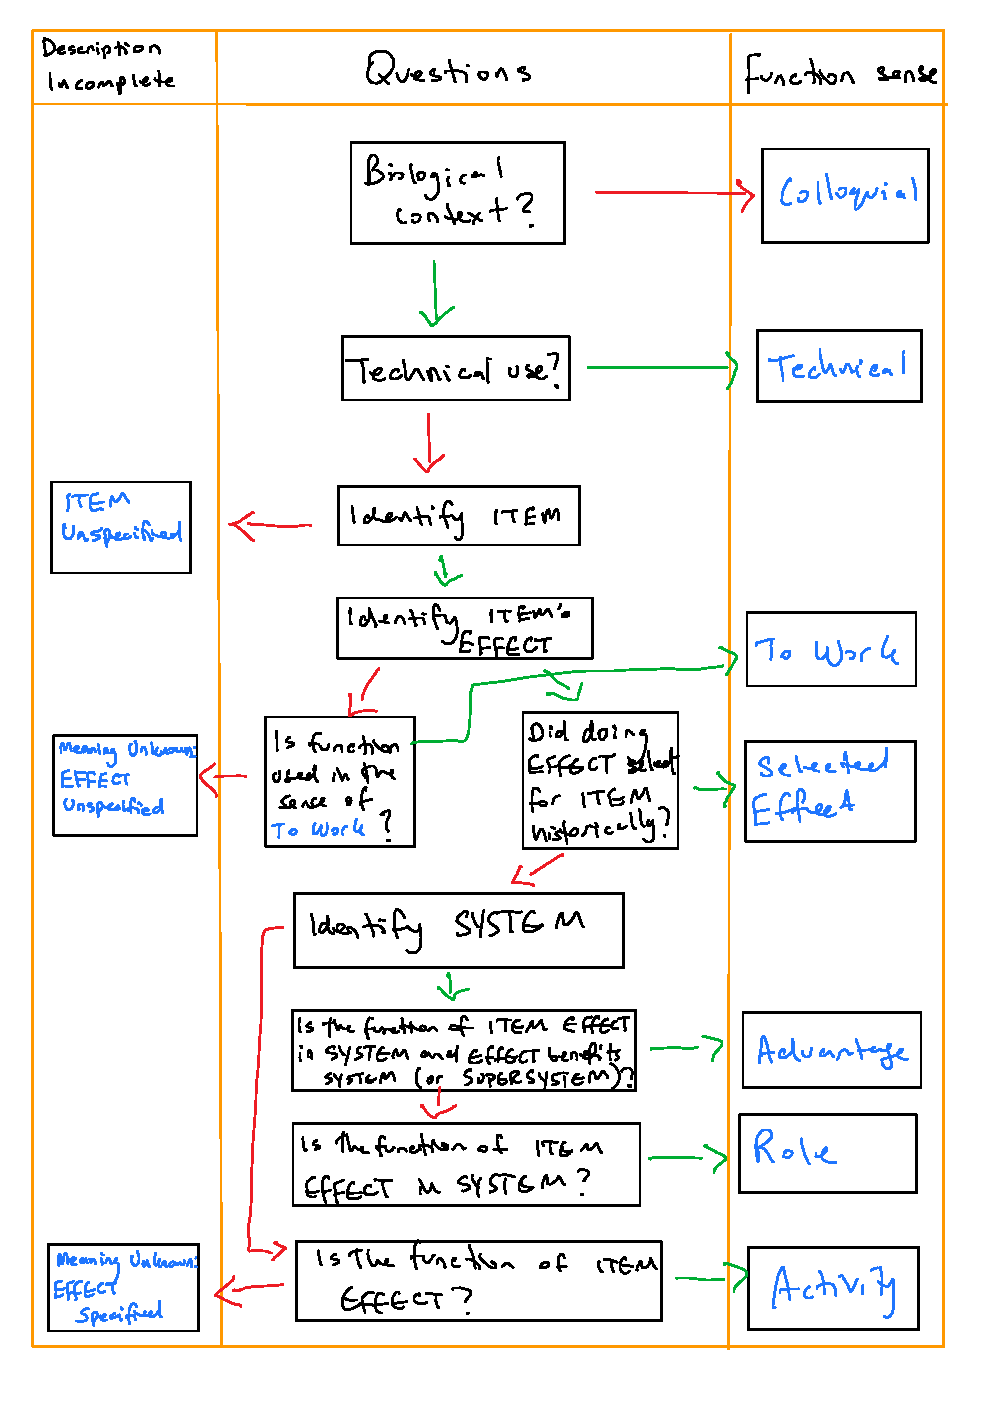
\includegraphics[width=\linewidth]{GeneralFlowchart.pdf}
  \caption[\textbf{Decision flowchart for identifying sense of function.}]{}
\end{figure}
\begin{landscape}
\begin{table}
  \begin{tabular}{|p{0.17\linewidth}|p{0.97\linewidth}|}
    \hline
    Decision point & Description \\
    \hline
    Biological context? & Are we dealing with a case of biological function or colloquial use? For a set of definitions of colloquial use, see \href{http://wordnetweb.princeton.edu/perl/webwn?s=function&sub=Search+WordNet&o2=&o0=1&o8=1&o1=1&o7=&o5=&o9=&o6=&o3=&o4=&h=}{WordNet 3.1}. Most colloquial senses will be rarely encountered if one has a sufficiently narrow corpus (i.e. limited to scientific publications). Notable exceptions are mathematical functions and programming functions, which we have included under colloquial for simplicity. \\
    \hline
    Technical use? & Compound phrases such as ``functional ecology'', ``functional biology'', ``functional connectivity'', and so on. These phrases will be familiar to practitioners within a field. Their meanings are multi-faceted and influenced by a field's development and cannot be meaningfully unpacked using a flowchart.  A useful heuristic is that these phrases will often appear multiple times throughout a manuscript. \\
    \hline
    Identify \emph{ITEM} &  An \emph{ITEM} is a noun (or noun phrase) that can be a character or trait of a Darwinian individual. This applies most obviously to concrete nouns like ``heart'' that refer to a physical item, but it can also include abstract nouns (denoting concepts, qualities, or states) if they refer to a concrete concept. For example, ``gene'' refers to the concept of an atomic unit of DNA that has a well-defined phenotypic effect. This is sufficiently concrete to qualify as a character even if it does not exactly map onto a physical piece of DNA. Importantly, there must be a grammatical dependence between function and the \emph{ITEM}---it is not merely sufficient that a suitable \emph{ITEM} appear somewhere in the sentence. For example, ``protein'', not ``muscle'', is the \emph{ITEM} in  ``protein function aids muscle development'' but ``muscle'', not ``protein'', is the \emph{ITEM} in ``protein aids in muscle function''. \\
    \hline
    Identify \emph{ITEM}'s \emph{EFFECT} & \emph{EFFECT} is what the \emph{ITEM} does (or, less commonly, has done to it). \emph{EFFECT} is a verb (or verb phrase if including associated modifiers). \emph{EFFECT} might not always act as a verb in the text, so long as it can be turned into a verb through word conversion (e.g. in ``contribute to transcription'', the noun ``transcription'' could be converted to the verb ``transcribe''). \\
    \hline
    Is function used in the sense of Perform? & A heuristic is whether you can substitute ``\emph{ITEM} function'' (or equivalent, depending on the sentence) with ``how well \emph{ITEM} performs'', ``a working \emph{ITEM}'' or similar into the raw sentence without loss of meaning. For example, ``Liver function is important for health'' might become ``A working liver is important for health'' without loss of meaning.\\
    \hline
    Did doing \emph{EFFECT} select for \emph{ITEM} historically? & Can it fit the following form: the function of \emph{ITEM} is to \emph{EFFECT} such that doing \emph{EFFECT} in the past caused \emph{ITEM} to be selected for or maintained in a population (relative to an actual or counterfactual historical alternative or set of alternatives to \emph{ITEM})? \\
    \hline
    Identify \emph{SYSTEM} & The \emph{SYSTEM} is a system that contains \emph{ITEM}. In the spirit of Cummins (1975), the \emph{EFFECT} of the \emph{ITEM} on the \emph{SYSTEM} contributes to an activity of \emph{SYSTEM}. As a heuristic for identifying \emph{SYSTEM}, you can ask questions such as "how does \emph{ITEM} produce \emph{EFFECT}?" or "for what is \emph{ITEM} producing \emph{EFFECT} used? \\
    \hline
  \end{tabular}
\end{table}
\end{landscape}

\section{Analysis of natural language}
\label{sec:analys-natur-lang}

Function has many derivatives (e.g. functional) and can be used in different parts of speech (noun, verb, etc.), which significantly complicates analysis of natural language.
If we focus just on the forms of function when used as a noun, we have the singular ``function'' (``the function of the heart''), and the plural ``functions'' (``the heart has many functions''), and the derivative ``functionality'' (``the functionality of the heart'').
Grammatical relations also vary.
In ``the function of the heart'' and ``the functionality of the heart'', function is the subject, whereas for ``the heart has many functions'', function is the direct object.
Aside from its use as a noun, ``functions'' (and ``function'') can also be used as a verb (``the heart functions to pump blood'').
We also encounter cases such as the gerund form ``functioning'', which is the -ing form of the verb ``function'' that acts as a noun (``functioning is important for hearts'')!
And to complicate matters even further, ``functioning'' might be a present participle instead of a gerund, in which case it either acts as an adjective (``the functioning heart'') or to form verb tense (``the heart was functioning''). Suffice it to say, when dealing with real-world sentences, the sheer variety of syntactical forms present a challenge for semantic interpretation of function.
Thus, the first component of our approach is to simplify these diverse syntactic constructions into common forms.
For example, a simple common form would be ``The function of \emph{x} is to \emph{y}'', where \emph{x} is a biological item (e.g. ``heart'') and \emph{y} indicates what the biological item does (e.g. ``pump blood'').

To simplify comparison of syntactically-diverse constructions, we will use word conversion to convert from derivations of "function" to its root form function (specifically morphological derivation and inflection). We will use morphological derivation to convert between parts of speech (e.g. adjective -> noun) and inflection to convert between number, tense and aspect (e.g. the plural functions to function). The key consideration during conversion is that we maintain (and convert if necessary) the dependencies between "function" and other parts of the sentence. What I will describe here is a method for converting these derivations of the word function to its base form (the verb or noun "function"), while at the same time, keeping track of and converting the form (where necessary) of the dependencies of "function". The idea is to rework the sentence such that semantic relations can be cast into a standard form.


\section{relevance for philosophy of medicine}
\label{sec:relev-phil-medic}

expand upon the ``performing'' category (I can put the bits about requiring some normative backing, dysfunction, etc. here)

\section{advice for best practices}
\label{sec:advice-best-pract}

should also mention that the elife paper has poor inter-observer agreement even though it overfits its definitions by testing on the ``train set''.

add some stuff on automation here and how some steps are better suited to statistical inference rather than rules (e.g. for selected effects and biological advantage it might be easier to label a bunch of examples and train a transformer model using supervision to classify the examples than it would be to provide bullet-proof rules)

\section{limitations and further considerations}
\label{sec:limitations}

- for simplicity ignored functions above the level of the individual (e.g. ecological functions)
- limit it to the sentence or to elsewhere in the document? First will make it easier to automate but latter might be more in-line with philosophical practices.
- even once you accurately categorise sentences, there's still the issue of how to classify documents. The distinction between ``this usage of function is of type x'' and ``these authors use function in manner y in this document''.

\section{example sentences}
\label{sec:example-sentences}

test=nlp("In general, these transcripts show little evidence of purifying selection, suggesting that many of them are not functional")

effect unspecified (Question: what have these transcripts done to cause them to be selected? Answer: we don't know, it's not specified)

change to

test=nlp("In general, these transcripts show evidence of translation into proteins, suggesting that many of them are functional")

either activity or role

change to

test=nlp("In general, these transcripts show little evidence of purifying selection on account of being translated into proteins, suggesting that many of them are not functional")

now selected effects

\section{Introduction-old-draft}
\label{sec:introduction-1}

-ENCODE and the debate
-Most biologists just talk of CR and SE but there are other types (activity (note Neander 2017 calls this minimal function), advantage, function-dysfunction)

describe the functions briefly but also include token type distinction and show how they're related (will need to reorganise a bit). determinable property (e.g. gene) and determinate property (e.g. allele) are both type-level properties. A particular allele in an individual would be a token-level property. (actually think the descriptions can go in the four questions bit. would be good to just start off with a high level description with some history/references)

Causal role function tends to talk of characters (or items or behaviours) and is interested in how they work within a complex system. It's mainly concerned with determinable types, as we want to talk about what this part or component does within a system. (Though I might need to do a little reading on this because Garson 2019 says that CR people consider a CR token being dysfunctional as being the same as having no function. I suppose CR need not be applied to types, as it doesn't have a lineage concept, but nevertheless it seems to be applied to types. For example, if a biologist runs an experiment, they use many individuals because they want to get at the type characterisation not token.)

Biological advantage function is causal role function with two differences: (i) it's comparative (trait $i$ vs trait $j$) and (ii) it's interested in variants of types (traits) rather than the characters themselves. BA functions answer the question ``what advantage does this trait variant give its bearer over another (counterfactual or actual) organism with a different trait variant?''.

Selected effects functions deal again with advantages of trait variants, only now it asks whether these advantages have accumulated in such a way that we can tell a causal story about how the effect of the trait variant has led to the evolution of the trait. A criticism of SE is that it doesn't tell you anything about the current function of the trait (see 2009 organizational closure paper), which is another argument for pluralism.

The functional-dysfunctional question deals with tokens---how has the trait evolved in the development of a particular individual? Although it must be said that this isn't the cleanest distinction. While we'll want to ascribe a dysfunctional state (e.g. disease) to an individual, we might cluster underlying etiologies into a single coarse grain phenotype (e.g. a syndrome). Might also cluster a single genotype change (e.g. mito diseases). This could also be without regard for trait (e.g. some mito diseases will apply to the character (all human mito haplotypes), though need to check that this is true), but perhaps some are specific to some traits.
Note that I think part of this comes down to the fact that it's not well-defined whether a new token is a new trait or whether it is a dysfunctional member of the type (i.e. are we dealing with a collection of dysfunctional tokens who are grouped based on either a common inheritance, common architecture, common phenotype, or a new trait type? (you could go via inheritance vs ontogeny but there might be some diseases that are hard to tease apart here? e.g. mito disease could be a mutation from mother, stable inheritance, mutation in zygote, etc.---would we really distinguish them if they're the same structurally? I need to be careful here because I'm claiming that dysfunction is ontogenic so I really need to be able to make the claim that dysfunction is token-level which means syndromes/diseases are collections of token dysfunctions. Note Neander 2017 says that malfunctions are token level.)
One way of talking about when a dysfunction becomes a trait is when it is heritable...this will lead to some odd cases (mitochondrial diseases becoming traits), or we just accept that harmful dysfunctions that are heritable are a grey zone. Huntington's disease is another good example because it can be caused by ``slippage'' of genetic repeats so is ontogenic in this sense, yet it is also heritable.
Neander (2017) actually seems to want to say that ``not performing function = malfunction'' due to mismatch (pg 1152)

EDIT 20201015

I want to split up the current utility case into a positive aspect (biological advantage) and a negative case (basically making the claim that because current utility contrasts traits, one can also talk about a biological disadvantage). Now of course for the negative case it doesn't provide an explanation for why something is there at least not in the biological advantage sense (it could be a SE that's no longer adaptive though). To fully explore the possibilities, I think we need to allow for biological disadvantage though (e.g. something that was selected for in the past but is now actively being selected against...e.g. a mismatch or something to do with the genetic architecture or development of the trait). While I already had this in the previous scheme, what's different now is the following. For \emph{some} of these cases of traits at a biological disadvantage, we will want to say that the traits are dysfunctional and that the carriers are diseased (e.g. sickle cell). This a way to get dysfunction at the trait (not token) level.

A second alteration is to let the functional-dysfunctional axis to be hyperfunctional-functional-dysfunctional. An individual's trait can perform its function (``functional''), it can fail to perform its function (``dysfunctional'') or it can perform its function better than expected (``hyperfunctional''). The latter might be due to plasticity (or even just random variation, such as with a ``lucky'' quantitative trait), or it might be due to a beneficial mutation, in which case it might lead to a new trait that will, in the future, be considered the wild type. Although I suppose that the latter case is technically not actually ontogeny (since the mutation occurs pre-fertilization), I chatted to Paul about this and he seems to think it would be fine to consider pre/post fertilization mutations as equivalent.

Will also need to address organizational theories and their claim of normativity. Will need to sidestep all the details but basically the main point is for dysfunction you need two things: (i) a Cummins-style functional analysis but of how an item is working in a token (not character); and (ii) a normative grounding that tells you how it ``ought to work''. All approaches must borrow elements from each other to make this work (SE needs CR; CR needs SE or some other framework that ascribes type-level normativity; organizational must borrow elements from CR and SE (for the latter need to see whether they've developed the reproduction aspect). So the point is that we need pluralism of the three function questions to get at dysfunction.

(This actually works well because it provides a nice justification for separating out the first three (types) for one framework and laying the last (token) over this framework.

also point out how SE function can generally only be established once we have ideas about CR and BA. The first thing we ask is ``what does this trait do?'' or ``how is this trait used?'' (actually these seem like the second thing; first thing should be ``how does it work?''); the second thing is ``what benefit does it provide to the organism?''; the third thing is ``might it have provided a benefit to the organism in the past?''; the fourth thing is ``can we explicitly show how the trait could have evolved due to its function(al effects)?''.
Although one might get away with just generically knowing what it does and hypothesizing an advantage (or even just knowing the advantage), without knowing details about how it works (e.g. genetic architecture, mechanism of action), it will be hard to build accurate models.
So with this I can basically deal with the issue I wanted to raise about how some (e.g. Garson) think that SE has greater explanatory power because they are, in part, conflating what we know because we know SE vs knowing all 3 (although obviously knowing SE is extremely important if you want to ask an evolutionary question)

another thing I can show is why many fields don't need to take an evolutionary approach to make accurate inferences, especially things to do with disease. I suspect here I can focus on the fact that disease is on the functional-dysfunctional continuum, which relates to how well a \emph{ahistorical} notion of function is working (i.e. CR or BA). It only relates to dysfunction of SE in the sense of dysfunction of a CR/BA doing what it was selected for (but even here the dysfunction relates specifically to the ahistorical CR function. So it follows that if we are interested in how something works or why somebody is diseased, then we don't necessarily need to know the evolutionary history (except how it relates to the present). It's also important to distinguish between SE dysfunction and the others. SE, being historical, can't dysfunction in the sense that it changes performance in a token whereas CR/BA dysfunction could (a CR instance having no function will have a similar phenotypic effect in a token to a CR instance having a function but being dysfunctional). If we define SE dysfunction as ``not being able to perform the CR for which it was selected for constitutional reasons'', then SE dysfunction is a broken CR mechanism in a selective/Normal environment. This is similar to what one might call a CR dysfunction, but note that garson would say that CR can't dysfunction because if a CR doesn't work then it doesn't have a function. I think I'll need to sidestep these issues and just focus on the fact that everybody would generally agree that dysfunction is when the trait is not ``working as it ought to'' with the ought to part being the source of most of the controversy.

note that the above case becomes much stronger if you subscribe to harmful dysfunction, as this puts even less emphasis on SE normativity.

Will need a section that looks at implicit use of other forms of function (e.g. CR functions assuming it leads to an advantage, BA functions assuming it will be selected for, SE functions taking for granting that CR/BA functions have been established, etc.)

Much argument seems to revolve around which conception of function is best. I will have shown that this misses the point: biologists and medical researchers want to be able to ask four function questions and no conception of function alone can currently serve this purpose.

mention that people might talk of something functioning in a disease but this is not the function of the thing (think Doolittle also made this point)

reason we want to know ontogeny as part of the four is that it would help us distinguish between an organism with a strong current utility but mildly dysfunctional trait and an organism with a weak current utility but fully functional trait

maybe point out that it's not useful to think of tinbergen's questions as two historical/two ahistorical (because although development is historical, it's over a timescale that is arguably shorter than the ahistorical notions of mechanism/utility) (probably just ignore this if possible though)

Character can be used to refer to a range of different biological items: a genetic sequence,
(Actually this is interesting. Technically a character should be a phenotype but then can we not talk of a gene as a character? Seems like if we can make a fairly straightforward genotype->phenotype mapping then we can do this, but if isn't? I'm trying to say that causal role functions are character-level but they need not be...we could just look at a transcription factor or something. So I guess the key point to make is that causal role functions need not be character level but they can be and are often employed in this manner.

causal/biological role---\textbf{mechanism}
biological advantage---\textbf{current utility}? (Nesse didn't like this but I think that's because he totally misunderstands what it actually is. I think it's fine because I agree that adaptive value will be misinterpreted more easily and Nesse is a case in point. Note that bekoff1995 used this term so it wasn't introduced by the 2013 tree paper)
selected effects---\textbf{evolution}
functional--dysfunctional---\textbf{ontogeny}

Function is used in a multitude of ways in the biological and medicine sciences.
There has been renewed interest in how function is used biology, in part due to debate over the ENCODE consortium and their annotation of functional elements of the human genome.
Several evolutionary biologists have weighed in on the debate (cite Doolittle, Graur), introducing some of the philosophical notions of biological function.
These have focused on two contrasting conceptions in function in particular: causal role and selected effects.
Causal role functions are utilised widely in fields like physiology, molecular biology, and genomics.
Causal role explanations view function as the mechanistic role that an item plays in a biological system.
Selected effects functions are primarily utilised in evolutionary biology (behavioural ecology?, some genetics?).
Selected effects explanations view functions as those effects of a trait that were selected for by natural selection.
Under this framework, a trait's function(s) is taken to constitute an explanation for the existence of the trait.
Although causal role and selected effects functions are the two concepts that have received the most attention from philosophers, there are a number of other notions.
In this paper, I show that the questions that philosophers address with their frameworks, and biologists address with their usage, can be cast into the familiar mould of Tinbergen's four questions.

\section{Function and the four questions}
\label{sec:funct-tinb-four}

Before I introduce function in the context of Tinbergen's four questions, I must first define some terminology, as philosophers and biologists often use quite different terms to refer to similar concepts.
One important distinction will be between what philosophers call \emph{types} and \emph{tokens}.
A type is a class of objects whereas a token is an instantiation of the class/type in an individual.
For example, the class ``chair'' is a type, but \emph{my} office chair is a token.
Philosophers further divide types into \emph{determinates} and \emph{determinables}.
A determinable property is a category that can be made more specific; a determinate property is a specific member of a determinable category. 
For example, the determinable property ``colour'' can be divided into the determinate properties ``red'' or ``blue''.
Now to translate these philosophical notions to biological terminology.
I will refer to a determinable (type) property of an organism as a \emph{character}, a determinate (type) property of an organism as a \emph{trait}, and a token property of a particular organism as a \emph{token trait}.
A character either refers to a phenotype or to an item that displays a phenotype, which includes behaviours, morphological features, production of biomolecules such as proteins and hormones, or even a genetic sequence (if there is a simple mapping to a phenotype).
A trait is a specific variant of a character, and a token trait is an instance of a trait in an individual.
For example, eye colour is a character, blue eyes is a trait, and \emph{my} blue eyes are a token trait.

\subsection{Mechanism: how does it work?}
\label{sec:mechanism}

A mechanistic analysis is applied to \emph{characters}.
One of the first questions we might ask of a character is ``how does it work?'' or ``what role does it play in an organism (or a system of the organism)?''.

We are generally not concerned here with traits.

Tinbergen denoted this question as ``causation'', but modern interpretations have preferred mechanism (cite bateson/laland).
This question is the domain of functional analysis, the name given to the approach from which we get causal role functions (cummins1975).
%Functional analysis, and therefore causal role functions, are closely intertwined with a reductionist approach to the scientific method.
It works roughly as follows.
An investigator chooses a complex biological system that has an interesting capacity (in the eyes of the investigator).
In the simplest case, she may analyse the system by reference to how its parts interact to produce said capacity.
If the system is particularly complex, she may break it down into various subsystems, and analyse the capacity of each of those subsystems with respect to how its parts interact.
This process can be recursively applied if the investigator wants to simplify the system further.
For example, let us say that the investigator is interested in how the cardiovascular system (system of interest) circulates blood and transports nutrients (capacity) in humans.
She can divide the cardiovascular system into subsystems (heart, lungs, blood vessels, etc.), each of which itself has a capacity and various parts.
Let's say she's interested how the heart (subsystem) pumps blood (capacity of subsystem).
Specifically, she wants to study how the heart's electrical conduction system's (subsubsystem) ability to regulate heart beat (capacity of subsubsystem) is affected by the Purkinje fibers's (subsubsubsystem) ability to conduct action potentials (capacity of a subsubsubsystem). (Should actually only go up to subsubsystem and then later show how you might break it down even more and design an experiment around it. Also need to be clearer on what is a system and what is a component...is there a difference? Finally, need to actually show how causal role functions assign functions---i.e. what are the functions in these examples---and give a compact definition.)
After doing so, she works her way back, taking the insights about how the Purkinje fibers affect the heart's electrical conduction system to better understand the heart.
Her better understanding of the heart in turn improves her understanding of the cardiovascular system ability to circulate blood and transport nutrients.
Although the terminology is laborious, this approach is consistent with how much biology is conducted and goes by many names: reductionism, mechanistic approach, or bottom-up approach.
Even a field like systems biology, which rejects the reductionist label, mechanistically model interactions between components of systems. (need to read up on this)



\subsection{Current utility: how is it used?}

Tinbergen denoted the second question as ``survival value'', but this term has fallen out of fashion because it highlights but one part of an organism's biological fitness.
I adopt the terminology of bateson/laland and call this current utility.

note that this is often called adaptive in biology

\subsection{Evolution: how did it evolve?}
\label{sec:evolution:-how-did}

note the connection with adaptation

\subsection{Ontogeny: how did it develop?}
\label{sec:ontogeny:-how-did}

% \begin{table}
% \centering
% \begin{threeparttable}
% \caption{Combining ``type'' notions of function to classify traits (note that this does not include the dimension of dysfunction)}

% \begin{tabular}{cccccc}
%   \multicolumn{3}{c}{Function categories}&
%   \multicolumn{1}{c}{}&
% \multicolumn{2}{c}{Biological description}\cr
% \cline{1-3}
% \cline{5-6}
% CR & BA & SE && Classification& Examples \\
% \hline

% \checkmark & \checkmark & \checkmark && Paradigmatic function & Heart pumping blood \\
% \checkmark & \checkmark & $\times$ && Exaptation & Feathers for flying \\
% \checkmark & $\times$ & \checkmark && Mismatch & Fat/sugar and obesity \\
% \checkmark & $\times$ & $\times$ && Nearly-neutral traits & biochemicaly-active junk DNA \\
% $\times$ & $\times$ & \checkmark && Vestigial & Human appendix,flightless bird wings, pseudogenes \\
% $\times$ & $\times$ & $\times$ && Spandrels/byproduct/parasitic DNA\tnote{1} & Transposable elements \\

% \hline

% \end{tabular}
% \begin{tablenotes}
% \item[1] Anything that was ``selected of'' rather than ``selected for'' (spandrels, byproducts, constraints) or something that was forced on an organism (e.g. viral DNA or transposable elements). The former evolved for other reasons and may not do anything for the organism while the latter primarily ``serves'' as a selfish element that is using the organism to spread its DNA.

% \end{tablenotes}

% \end{threeparttable}
% \end{table}

\section{Conclusion}
\label{sec:conclusion}

Note that biologists sometimes confuse a weaker notion of mechanism with causal role.
ENCODE's definition of function, for example (and Grauer, etc mischaracterisation of CR)
(This isn't straightforward, because ENCODE's definition doesn't really deal with characters. I might just need to deal with this at the end.)


\end{document}
%%% Local Variables:
%%% mode: latex
%%% TeX-master: t
%%% End:
